\fancyhead[LE,RO]{\itshape CAPÍTULO \arabic{chapter}}
\fancyhead[LO,RE]{\itshape \rightmark}
\chapter{Homotopía: Nociones básicas}\label{sec:homotbas}
\fancyhead[LO,RE]{\itshape 1.0. NOCIONES BÁSICAS}
La relación de homotopía es básica y formaliza la noción de deformación continua de dos espacios: 
\begin{defin}
Dos aplicaciones $f, g : X \longrightarrow Y$ se dicen homótopas (deformables la una en la otra), denotado por $f \simeq g$, si existe  $H : X \times [0,1] \longrightarrow Y$ una aplicación tal que $H(x ,0) = f(x)$ y $H(x, 1) = g(x)$.
\end{defin}
\begin{prop}
La relación de homotopía es una relación de equivalencia en el conjunto de aplicaciones continuas de $X$ a $Y$.
\end{prop}
\begin{demo} 
La propiedad reflexiva es clara sin más que tomar la aplicación $F(x,t) = x$.\\
Para la simétrica, si $H : f \simeq g$ entonces $F : X \times I \longrightarrow Y$, $F(x, t) = H(x, 1-t)$ es una homotopía de $g$ a $f$.\\
Veamos ahora la transitiva. Si $F : f \simeq g$, $H : g \simeq h$ entonces $G : X \times I \longrightarrow Y$,

$$G(x, t) = 
\begin{cases}
	F(x, 2t) 	& 	\text{ si } t \leq \frac{1}{2},\\
	H(x, 2t - 1)& 	\text{ si } t \geq \frac{1}{2},
\end{cases}$$ 
es una homotopía de $f$ a $h$.
\end{demo}
\begin{ejems}
\begin{enumerate}
\item \label{ej1:1} Cuando $X = I$, esto es, al trabajar con curvas, se observa mejor la deformación:
\begin{figure}[h]
\centering
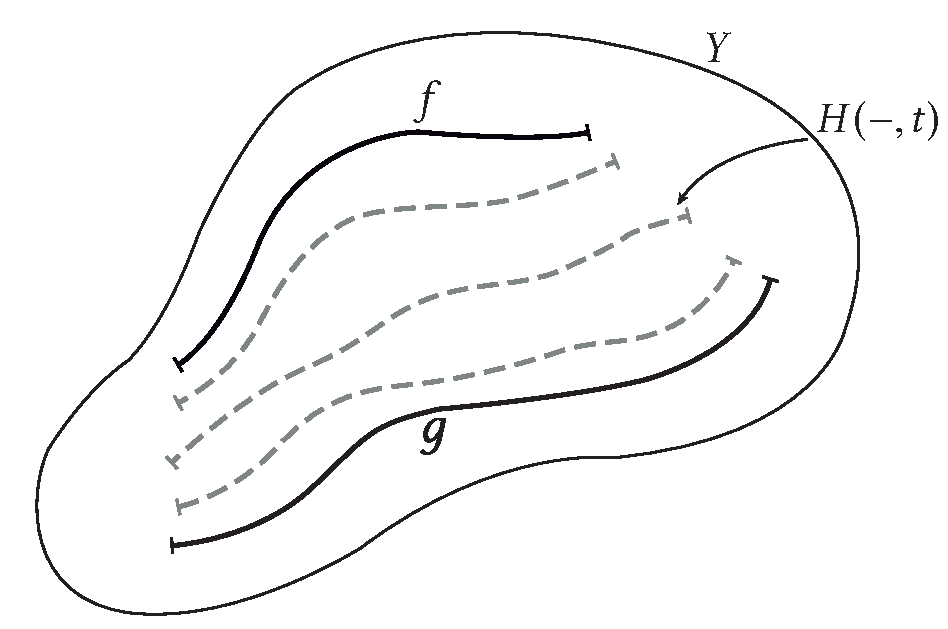
\includegraphics[width=0.4\textwidth]{images/homotcamin.pdf}
\end{figure}
\item \label{ej1:2} \hypertarget{ej1:2} Sean $X = Y = \mathbb{R}^n$, y consideremos las aplicaciones $f = Id_{\mathbb{R}^n}$ y $g \equiv 0$. Entonces $f \simeq g$ mediante la aplicación
\begin{align*}
H : \mathbb{R}^n \times I &\longrightarrow \mathbb{R}^n, \\
H(x, t) &= tx.
\end{align*}
\end{enumerate}
\end{ejems}
A menudo estamos interesados en aplicaciones entre pares
\[f : (X, A) \longrightarrow (Y, B), \]
la cual definimos como una aplicación continua tal que $f(A) \subset B$. En este caso, $f, g : (X, A) \longrightarrow (Y, B)$ son homótopas si existe $H : X \times I \longrightarrow Y$ tal que 
\[
H_t = \nobreak H(-, t) : (X, A) \longrightarrow (Y, B) \quad \forall t \in I.
\]
Un caso particular de suma importancia es el de los espacios punteados $(X, x_0)$. En este caso, $f \simeq g : (X, x_0) \longrightarrow (Y, y_0)$ si existe $H: X \times I \longrightarrow Y$ tal que $H(x, 0) = f(x), H(x, 1) = g(x)$ y $H(x_0, t) = y_0$ $\forall t \in I$.\\
\begin{ejems}
\begin{enumerate}
\item \label{ej2:1} En el ejemplo anterior \ref{ej1:2}, podemos considerar $f \simeq g : (\mathbb{R}^n, 0) \longrightarrow (\mathbb{R}^n, 0)$, tomando como homotopía la misma función $H$.

\item \label{ej2:2} Si consideramos un espacio como el siguiente: \\
\begin{tabular}{ll}
\begin{minipage}{0.5\textwidth}
Tenemos que $f : I \longrightarrow Y$ es obviamente homótopa a la constante en $y_0$ que denominamos $c_{y_0}$. Pero la aplicación de pares $f : (I, \{ 0,1 \}) \longrightarrow (Y, y_0)$ no es homótopa a la constante $c_{y_0}$.
\end{minipage}
&
\begin{minipage}{0.5\textwidth}
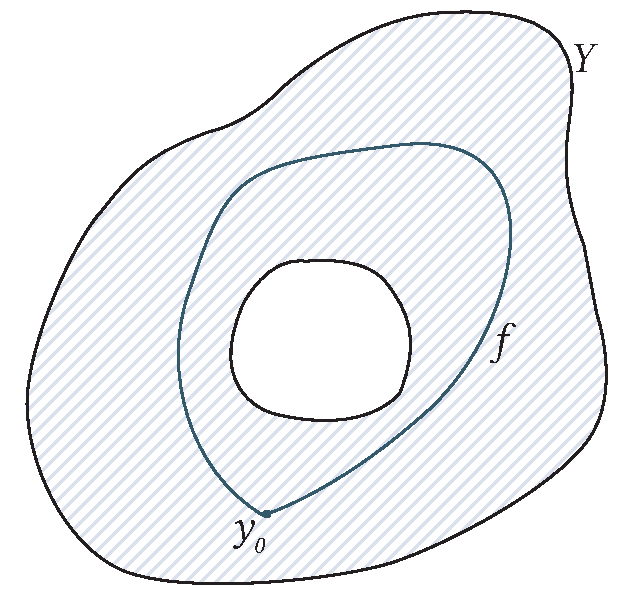
\includegraphics[width=0.65\textwidth]{images/homotrelatalt.pdf}
\end{minipage}
\end{tabular}

\item \label{ej2:3} Dado $D^2 = \{ x \in \mathbb{R}^2 : \| x \| \leq 1 \}$, tenemos que $Id \simeq a$ donde $a$ es la función antípoda mediante la hopotopía de la rotación: $H : D^2 \times I \longrightarrow D^2$ dada por $H(x, t) = H(\rho e^{i\theta}, t) = \rho e^{i(\theta + t\pi)}$. \par
\begin{figure}[h]
\centering
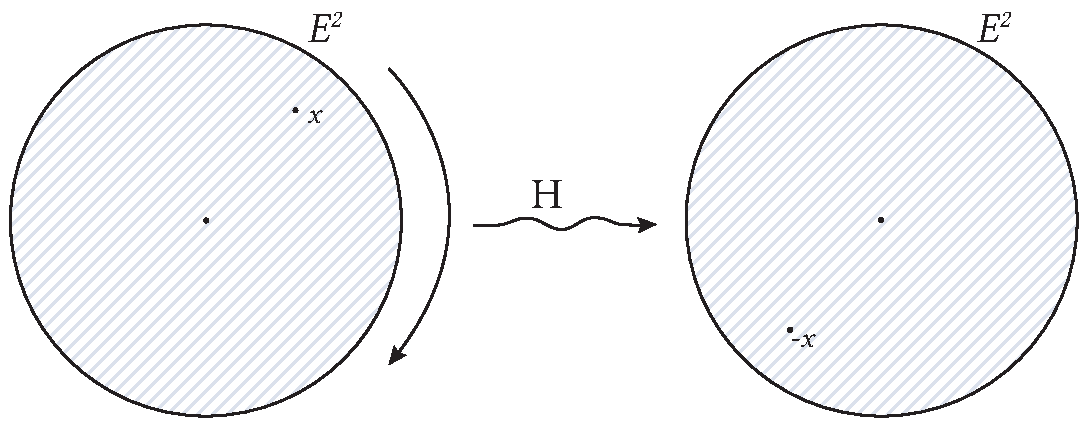
\includegraphics[width=0.65\linewidth]{images/homotrotacalt.pdf}
\end{figure}
Como aplicaciones de pares, $Id \simeq a$ mediante $H : (D^2, S^1) \times I \longrightarrow (D^2, S^1)$. Sin embargo, no existe ningún punto $x_0 \neq 0$ tal que $Id \simeq a$ como aplicaciones $(D^2, x_0) \longrightarrow (D^2, x_0)$.
\end{enumerate}
\end{ejems}
Al conjunto cociente formado por las clases de homotopía de aplicaciones continuas de $(X, A)$ en $(Y, B)$ se le denota por $[(X, A), (Y, B)]$. \par

Veamos ahora la definición de que dos espacios sean ``deformables'' el uno en el otro:

\begin{defin}
Dos espacios $X$ e $Y$ son homotópicamente equivalentes si existen aplicaciones $f: X \longrightarrow Y$ y $g: Y \longrightarrow X$ tales que $g \circ f \simeq 1_X$ y $f \circ g \simeq 1_Y$. A las aplicaciones $f$ y $g$ se les denomina equivalencias de homotopía.
\end{defin}

\begin{ejems}
\begin{enumerate}
\item \label{ej3:ret} \textbf{Retractos}: La aplicación $A \stackrel{i}{\longhookrightarrow} X$
es un retracto de X si existe una aplicación $r : X \longrightarrow A$ tal que $r \circ i = 1_A$.
Decimos que $A$ es un retracto de deformación de $X$ si además $i \circ r \simeq 1_X$.\par
Como ejemplo, $S^n = \{ x \in \mathbb{R}^{n+1}$ : $\| x \| = 1 \}$ es un retracto de deformación de $\mathbb{R}^{n+1} -\{ 0 \}$. En efecto, si consideramos 
\begin{align*}
r : \mathbb{R}^{n+1} &-\{ 0 \} \longrightarrow S^n, \\
x &\longmapsto \frac{x}{\| x \|},
\end{align*}
entonces 
\begin{align*}
H : \mathbb{R}^{n+1} -\{ 0 \} &\times I \longrightarrow \mathbb{R}^{n+1} -\{ 0 \}, \\
H(x, t) &= (1 - t)x + \frac{tx}{\| x \|} ,
\end{align*}
es una homotopía entre $Id_{\mathbb{R}^{n+1} -\{ 0 \}}$ e $i \circ r$.

\item \label{ej3:contr} \textbf{Espacios contráctiles}: Un espacio X es contráctil si tiene el mismo tipo de homotopía de un punto, o equivalentemente, la identidad en $X$ es homótopa a una constante. Por ejemplo, como hemos visto en \hyperlink{ej1:2}{uno de los ejemplos anteriores}, $R^n$ y $D^n$ son espacios contráctiles.

\item \label{ej3:peine} \textbf{El espacio peine} P es un espacio contráctil. P es el conjunto definido de la siguiente forma: 

\begin{tabular}{ll}
\begin{minipage}{0.3\textwidth}
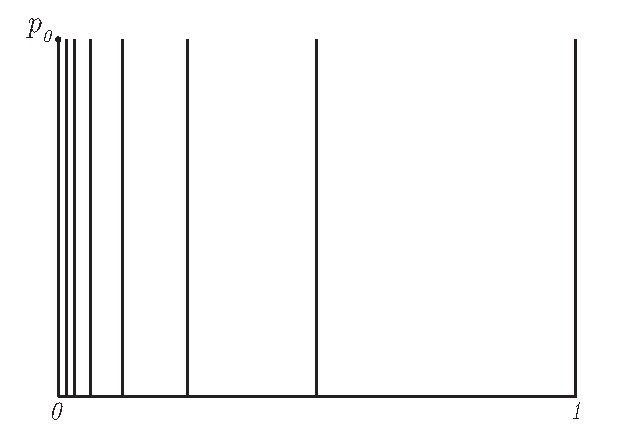
\includegraphics[width=\textwidth]{images/peine.pdf}
\end{minipage}
&
\begin{minipage}{0.6\textwidth}
\[ P = \bigcup_{n=1}^\infty \left( \left\lbrace \frac{1}{n} \right\rbrace \times [0, 1]\right) \cup \{ 0 \} \times [0, 1] \cup [0, 1] \times \{ 0 \}, \]
que obviamente es contráctil, aunque $Id_P \not \simeq_{p_0} c_{p_0}$ para un $p_0 \notin [0, 1] \times \nobreak \{ 0 \} $.
\end{minipage}
\end{tabular}
\end{enumerate}

\end{ejems}
Relacionado con el ejemplo \ref{ej3:contr} y con el problema de la extensión tenemos el siguiente resultado:\\
\begin{teor}
Sea $f : S^n \longrightarrow X$ una aplicación continua. Entonces $f$ es homótopa a una constante si y sólo si $f$ se extiende al disco:
\[
\begin{tikzcd}
	S^n \arrow{rr}{f} \drar[hook, swap]{i} & & X \\
		& D^{n+1} \urar[swap]{\tilde{f}} & .
\end{tikzcd}
\]
\end{teor}
\begin{demo}
Supongamos $H : f \simeq c_{x_0}$. Definimos entonces $\tilde{f} : D^{n+1} \longrightarrow X$ dada por:
\[
\tilde{f}(p)= 
\begin{cases}
	x_0 & \text{ si }\| p \| \leq \frac{1}{2}, \\
	H(\frac{p}{\| p \|}, 2 - 2\| p \|) & \text{ si } \| p \| \geq \frac{1}{2},
\end{cases}
\]
que es la extensión que queríamos.

Recíprocamente, si $\tilde{f}$ es una extensión, $H(x, t) = \tilde{f}((1 - t)x)$ es una homotopía de $f$ a la constante. 
\end{demo}

\section{Espacios comúnmente utilizados}\label{c1:espcomun}
\fancyhead[LO,RE]{\itshape \rightmark}
Algunas de las construcciones que son de gran utilidad son las siguientes:
\begin{itemize}
\item \hypertarget{ecom:prod}{\textbf{El producto de espacios}} $X \times Y$.

\item \hypertarget{ecom:suma}{\textbf{La suma puntual}} o ``wedge'', denotado por $X \vee Y$ que puede verse como el conjunto cociente $\faktor{X \dot\cup Y}{\scriptstyle x_0 \sim \nobreak y_0}$ o como un subconjunto de  $X \times Y$, esto es, 
\[X \vee Y = X \times \{y_0\} \cup \{x_0\} \times Y.\]

\item \hypertarget{ecom:smash}{\textbf{El smash}} definido como 
\[ X \wedge Y = \faktor{X \times Y}{X \vee Y.}
\]
Esto es, el producto en el que identificamos ``los ejes'' a un punto.


\begin{tabular}{ll}
\begin{minipage}{0.5\textwidth}
\item \hypertarget{ecom:cono}{\textbf{El cono de $X$.}} Dado un espacio topológico $X$, el cono de $X$ se define como 
\[
CX = \faktor{X \times I}{X \times \{0\}.}
\]
Si queremos puntear el espacio, hacemos además
\[CX = \faktor{X \times I}{X \times \{ 0 \} \cup \{ x_0 \} \times I} \] 
\end{minipage}
&
\begin{minipage}{0.5\textwidth}
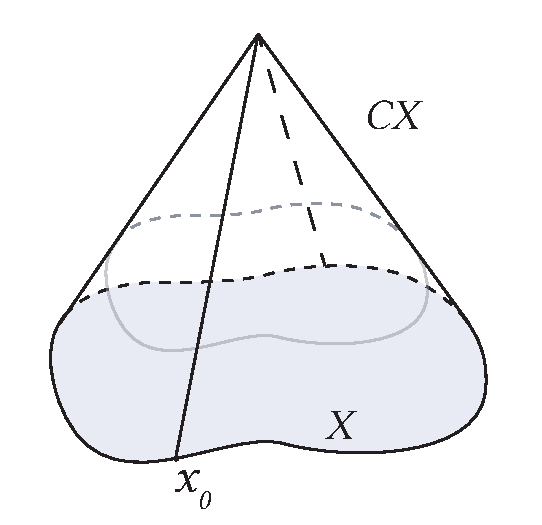
\includegraphics[width=0.6\textwidth]{images/conox.pdf}
\end{minipage}
\end{tabular}
 
 donde el punto base es $[x_0, t]$. La aplicación 
\begin{align*}
X &\longhookrightarrow CX, \\ 
x &\longmapsto [(x, 1)],
\end{align*}
es un homeomorfismo en su imagen por lo que podemos pensar en $X$ como un subespacio del cono. Además, el espacio $CX$ es contráctil.
\end{itemize}
\section{Adjunción de celdas a un espacio}\label{c1:unionceldas}
Sea $X$ un espacio topológico y $D^n$ un disco de dimensión $n \geq 1$. 
 Sea $f : S^{n-1} \longrightarrow X$ una aplicación continua. Definimos $X \cup_f e^n$, el espacio obtenido adjuntando a X una $n$-celda mediante $f$, como \par
\begin{tabular}{ll}
\begin{minipage}{0.5\textwidth}
\[ X \cup_f e^n := \faktor{ X \: \dot{\cup} \: D^n}{ \sim} \: , \]
\end{minipage}
&
\begin{minipage}{0.5\textwidth}
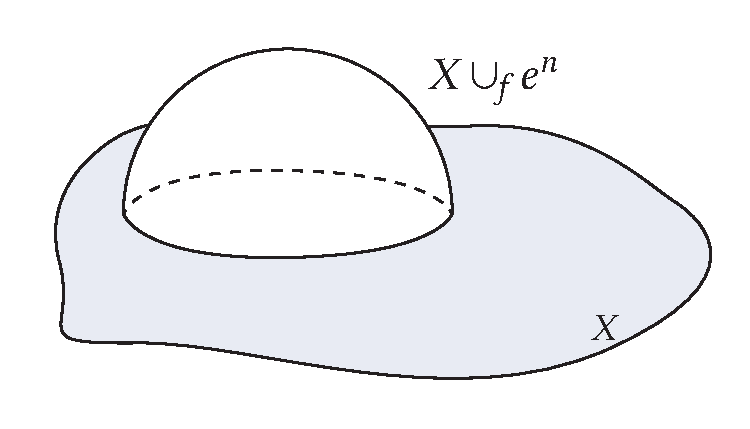
\includegraphics[width=0.8\textwidth]{images/uceldas.pdf}
\end{minipage}
\end{tabular}
donde $\sim$ es la menor relación de equivalencia que contiene a $x \in S^{n-1} \sim f(x)$.

\begin{prop}
La adjunción de una celda sólo depende del tipo de homotopía de la aplicación de adjunción.
\end{prop}
\begin{demo}
Sean $f , \, g : S^{n-1} \longrightarrow X$ dos funciones con el mismo tipo de homotopía, $f \simeq g$. Veamos que entonces que $X \cup_f e^n \simeq X \cup_g e^n$.\par 
Si $H : f \simeq g$, definimos las siguientes funciones:
\[
k : X \cup_f e^n \longrightarrow X \cup_g e^n
\text{ dada por }
k(x) = 
\begin{cases}
	x  & \text{si } x \in X, \\
	2x & \text{si } x \in e^n$, $\| x \| \leq \frac{1}{2}, \\
	H(\frac{x}{\| x \|}, \, 2 - 2\|x\|) & \text{si } \| x \| \geq \frac{1}{2}.
\end{cases}
\]
$$h : X\cup_g e^n \longrightarrow X \cup_f e^n
\text{ dada por }
h(x) = 
\begin{cases}
	x  & \text{si } x \in X, \\
	2x & \text{si } x \in e^n$, $ \| x \| \leq \frac{1}{2}, \\
	H(\frac{x}{\| x \|}, \, 2\| x \| - 1) & \text{si } \| x \| \geq \frac{1}{2}.\\
\end{cases}$$
Y tenemos que $h \circ k \simeq 1_{X \cup_f e^n}$ mediante la función $F : X \cup_f e^n \times I \longrightarrow X \cup_f e^n$ dada por: \\
\[
F(x,t) = 
\begin{cases}
	x  & \text{si } x \in X, \\
	4x & \text{si } \| x \| \leq \frac{1}{4}, \\
	H(\frac{x}{\| x \|}, (4\|x\| - 1)t) & \text{si } \frac{1}{4} \leq \| x \| \leq \frac{1}{2}, \\
	H(\frac{x}{\| x \|}, (2 - 2\|x\|)t) & \text{si } \| x \| \geq \frac{1}{2}.
\end{cases}
\]
De forma análoga se prueba que $k \circ h \simeq 1_{X \cup_g e^n}$.
\end{demo}
\begin{coro}
Si $X$ es arcoconexo, $X \cup_f e^1 \simeq X \vee S^1$ y si $f$ es homótopa a una constante (o nulhomótopa), entonces
$X \cup_f e^n \simeq X \vee S^n$. \qed
\end{coro}
\newpage
\begin{teor}
Una aplicación $f : (X, x_0) \longrightarrow (Y, y_0)$ es nulhomótopa si y sólo si se extiende a $CX$: 
$$
\begin{tikzcd}
	X \arrow{rr}{f} \drar[hook] & & Y \\
	& CX \urar[dashed, swap]{h} &  .
\end{tikzcd}
$$
\end{teor}
\begin{demo}
Sea $H : f \simeq c_{y_0}$ una homotopía. Definimos entonces la aplicación $h : CX \longrightarrow Y$, dada por $h([x, t]) = H(x, t)$. Está bien definida, ya que se tiene que  $H(X \times \{ 0 \} \cup \{ x_0 \} \times I) = y_0$ y se extiende a $f$.\par 
Recíprocamente, dada $h : (CX, \ast) \longrightarrow (Y, y_0)$ extensión de $f$, definimos una homotopía $H: X \times I \longrightarrow Y$ como $H = h \circ \pi$ (donde $\pi: X \times I \longrightarrow CX$ es la proyección canónica) y se tiene que 
$H(x, 0) = y_0$, $H(x, 1) = f(x)$ y $H(x_0, t) = y_0$.
\end{demo}

\section{Dualidad de Eckmann-Hilton}
Este principio de dualidad, en su forma más básica, consiste en la idea de, dado un diagrama para una construcción, invertir el sentido de las flechas de dicho diagrama. \par 
Un ejemplo de esto son las fibraciones y cofibraciones. Estas dos construcciones son duales en el sentido de Eckmann-Hilton. \par
Una fibración $p : E \longrightarrow B$ verifica que posee la HLP, que se representa por el diagrama:
\[
\begin{tikzcd}
X \arrow{rr}{g} \arrow[hook, swap]{dd}{i_o} &  & E \arrow{dd}{p} \\
\\
X \times I \arrow{rr}[swap]{G} \arrow[dashed]{uurr}{\widetilde{G}} & & B
\end{tikzcd}
\]
Y una cofibración $i : A \longrightarrow X$ es tal que posee la HEP, que viene dada por el diagrama:
\[
\begin{tikzcd}
	{} 						  & X \drar{i_0} \arrow[bend left]{drr}{f}			   &        					&   \\
	A \urar[hook] \drar{i_0}  &   												   & X \times I \rar[dashed]{F} & Y \\
	   						  & A \times I  \urar[hook] \arrow[bend right]{urr}{G} &   							&
\end{tikzcd}
\]
Éste último diagrama podemos cambiarlo haciendo uso de la identificación entre aplicaciones de $X \times I$ en  $Y$ con aplicaciones de $X$ en $Y^I$. Así, tendríamos que el diagrama queda de la siguiente forma:\[
\begin{tikzcd}
Y & & X \arrow{ll}[swap]{f} \arrow[dashed]{ddll}{\widetilde{F}} \\
\\
Y^I \arrow[two heads]{uu}{\pi} & & A \arrow[hook,swap]{uu}{i} \arrow{ll}{G}
\end{tikzcd}
\]
En el cual se ve que el sentido de las flechas es el contrario que en la fibración. \par
%Además esto también se observa entre las sucesiones exactas dadas por fibraciones y cofibraciones: \par
%Para una cofibración, teníamos la sucesión de Barratt-Puppe:
%\[ X \longrightarrow Y \longrightarrow C_f \longrightarrow \Sigma X \longrightarrow \Sigma Y \longrightarrow \Sigma C_f \longrightarrow \Sigma^2 X \longrightarrow \dots \]
%Y para las fibraciones teníamos la sucesión dada por la fibra homotópica de una aplicación:
%\[ \dots \longrightarrow \Omega^2 Y \longrightarrow \Omega F \longrightarrow \Omega X \longrightarrow \Omega Y \longrightarrow F \longrightarrow X \longrightarrow Y \]